\todo[inline]{The current thinking goes as follows


	* This is the methods section.  
	
	* The methods describes the tools and what we did.  
	
	* First the system (including interface?).  
	
	* Then the data.  
	
	* Then what we did with the data.}  

\subsection*{TOTUS system}
The TOTUS system consists of a set of services built around a geospatial database following a client-server architecture. Figure \ref{fig:system_diag} shows a high level diagram of the sistem highlighting its main components.
\begin{itemize}
	\item \textbf{Data store}: The database sitting at the core of the TOTUS system is implemented using PostgreSQL 9.2 \cite{pgsql} with PostGIS 2.0 \cite{postgis}. The data schemas are aimed at giving TOTUS the necessary flexibility to deal with different data sources. Figure \ref{fig:db_diag} shows the overall structure of the spatial database. The assessment modules implemented in the database are described in the following subsections. The database can be accessed directly or through the system's access layer.
	\item \textbf{Access layer}: An instance of FeatureServer\cite{dummy_temp}\todo{citation needed FeatureServer} enables the system to be accessed using OGC standard compliant clients through the Web Feature Service (WFS) of the Open GIS
	Consortium (OGC) for querying the underlying data sets.
	\item \textbf{Presentation layer}: To facilitate the interaction with the system and provide potential users with a preview of its capabilities, a simple web interface was developed that showcases key functionalities of the system.
\end{itemize}

The code is released under the GPL(?) license and it is available in the project's GitHub page\todo{ref code repo}

\begin{figure}
	\caption{TOTUS system overview}
	\label{fig:system_diag}
	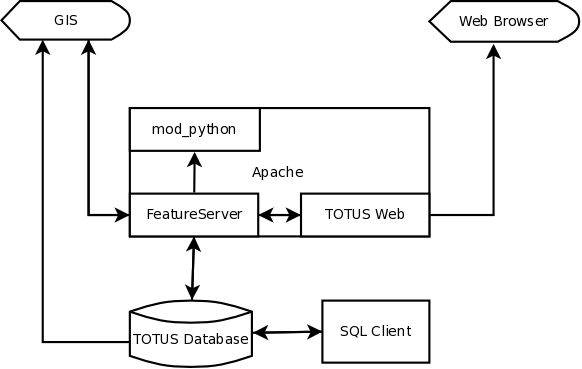
\includegraphics[width = 12cm]{system.png}
\end{figure}

\begin{figure}
	\caption{TOTUS database overview}
	\label{fig:db_diag}
	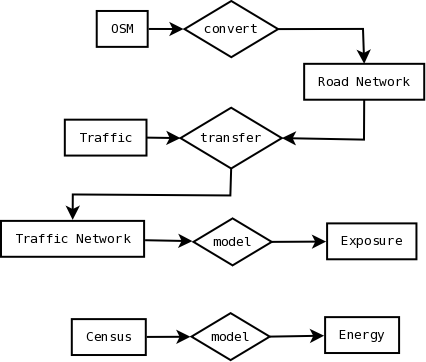
\includegraphics[width = 12cm]{system_data.png}
\end{figure}

\subsubsection*{TOTUS Modules}
\todo[inline]{brief introduction to the modules section}
The modular approach followed in TOTUS delivers the necessary flexibility when dealing with different data sources and also enables the update and upgrade of individual components as the research advances. The details of the implementation of the database modules can be found in TOTUS code repository\cite{dummy_temp}\todo{code repo}

\subsubsection*{Routing engine}
A key component of the TOTUS system is its routing engine. Implemented based on pgRouting (vXX\todo{pgRouting version?})\cite{dummy_temp}\todo{citation needed pgRouting}, This module enables some of the most powerful features in TOTUS like trip-dependent exposure and energy calculations as well as route optimisation based on arbitrary cost functions (e.g., minimum energy, minimum exposure, maximum \textit{enjoyment}, etc.). From a scenario evaluation point of view, the advantages of the database routing approach for TOTUS are that the spatial data and attributes can be modified and any data changes can be reflected instantaneously through the routing engine. The implementation of this module takes a streamlined version of the Open Street Map \cite{dummy_temp}\todo{OSM ref} data schema and converts it into a directed graph using \textit{osmosis}\cite{dummy_temp} and \textit{osm2pgrouting}\cite{dummy_temp}. The routing information is kept on a separate data schema that can be linked to the physical road network by the unique OSM feature identifier.

\subsubsection*{Exposure}
The current version of TOTUS' exposure module is based on a \textit{Traffic Impact Factor} developed by Longley et al\cite{dummy_temp}\todo{Citation needed TIF} to model NO$_2$ on a arbitrary grid. The method calculates, for a given point, an estimate of the impact of traffic from all the roads in the domain. This is applied to the centres of the cells that form the desired grid. The following diagram describes the calculations. For more details see Longley et al\cite{dummy_temp}\todo{Citation needed TIF}

\begin{equation}
TIF_{x,y} = \sum_{road=1}^{R}{(Length_{road}*Traffic_{road})^{exp}}
\end{equation}


\subsubsection*{Energy}

This module enables the implementation of an energy consumption calculator for any arbitrary census area (from meshblock to country) based on any arbitrary metric available for such census area. The implementation of the energy consumption model is flexible and allows for the interactive generation of various scenarios. 

In simple terms, the module only stores the \textit{metadata} needed to configure a model run in terms of its identifier ( \textit{activity} and \textit{scenario}) and the specific model definition (and its parts). The definition is stored in the \textit{model\_definition} table while \textit{model\_definition\_part} defines the individual parts of the equation (see Equation \ref{eq:energy}) that are aggregated to produce a final intensity
value. Each model definition part is described by a demographic data and the coefficient to apply. Figure \ref{fig:energy_diag} shows an overview of the Energy data schema.

\begin{equation}
\label{eq:energy}
EI=\sum_{parts}{CensusData_1*C_1+CensusData_2^{C_2}}
\end{equation}


\begin{figure}
	\caption{Energy schema overview}
	\label{fig:energy_diag}
	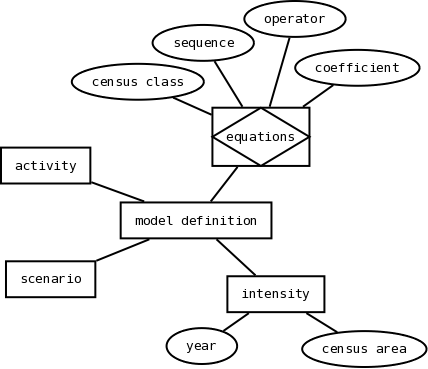
\includegraphics[width = 12cm]{energy.png}
\end{figure}

\subsubsection*{Emissions}
By extending the use of the \textbf{Energy} module, the Emissions and Socio-economic Model (ESESM)\todo{Wilton, E., Baynes, M., Bluett, J. (No date) Good practice guide for designing and implementing an incentive programme for domestic heating. Report prepared under the Envirolink Tools project nember NIWX0802, Environet and NIWA, 171p.} was implemented. The formulation\todo[inline]{This needs finishing ... describe what we did and how}

\subsection*{System Set Up}
%\subsubsection{TOTUS data store setup}
%Figure \ref{fig:totus_setup_flow} shows the workflow to setup the data store for TOTUS.
%\begin{landscape}
%	\begin{figure}[h]
%		 \caption{TOTUS setup workflow}
%		 \label{fig:totus_setup_flow}
%		 \missingfigure{Workflow diagram for TOTUS setup and data loading}
%		  %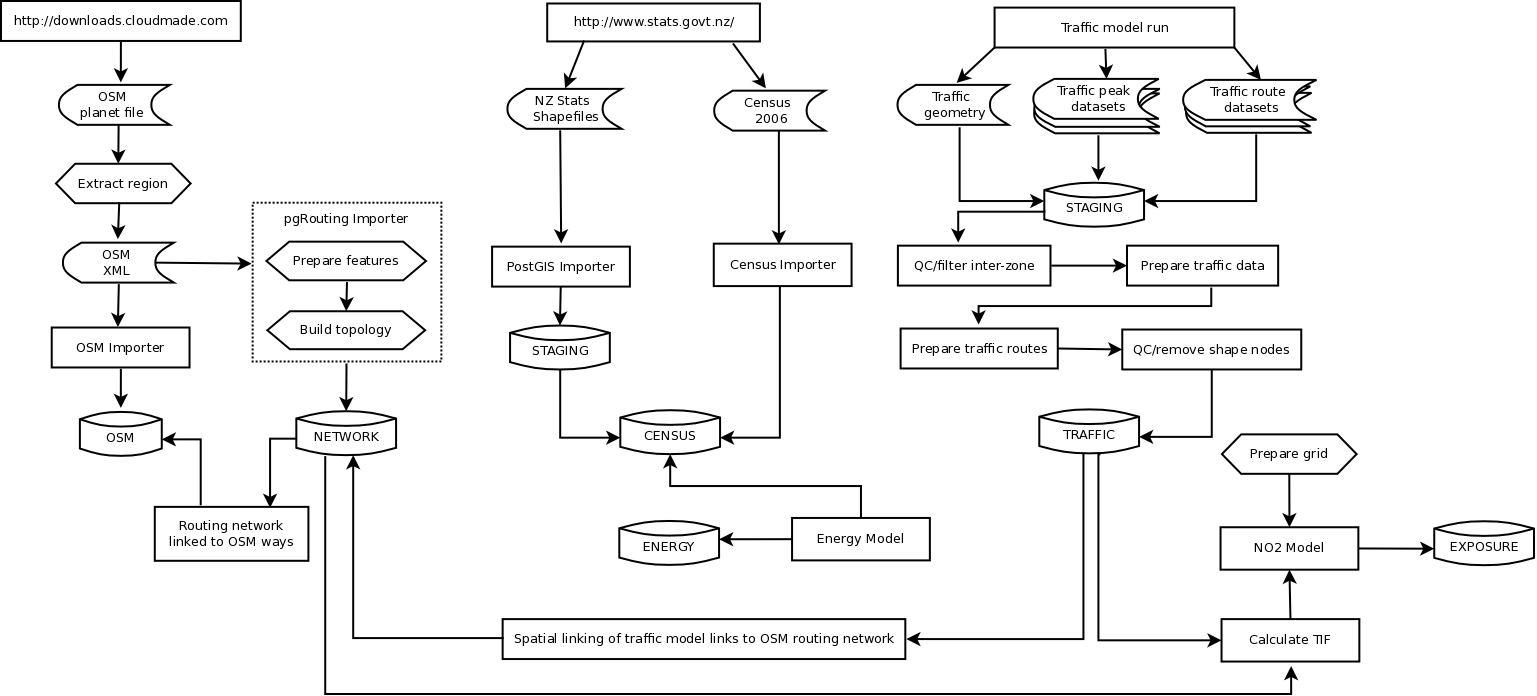
\includegraphics[width=\linewidth]{./system_preparation.png}
%		   % system_preparation.png: 1537x696 pixel, 51dpi, 76.85x34.80 cm, bb=0 0 2178 986
%	\end{figure}
%\end{landscape}

The primary data source of TOTUS is the Open Street Map (OSM) dataset. The TOTUS
loader requires an OSM \textit{planet file} for the area of interest. These data are then imported to the \textit{osm}  and \textit{network} schemas.  All routing edges (\textit{network}) are linked with their OSM counterparts to allow modifications of the OSM to used any other attributes or spatial features of interest to TOTUS.

The next step is to load the traffic model dataset defined to be compatible with traditional strategic traffic modelling packages (EMME, CUBE, etc). This dataset consists of two set of files. The first is shape files defining the traffic model zones and the modelled links both in terms of their geometry and their attributes. The second one is spreadsheets that contain all the traffic attributes for each link and for each traffic period modelled. Although not required, public transport information can be loaded in a similar fashion to traffic modelling data.

Once the traffic model data is loaded, it needs to be linked to the \textit{osm} schema. This is not a trivial exercise if the \textit{links} in the traffic model do not accurately represent the geometry of the road network. The linking process used in TOTUS is described elsewhere\cite{dummy_temp}\todo{MAKE THIS REFERENCE APPEAR!!!}. 

Finally, the census data, provided as spreadsheets, is loaded using the TOTUS census importer. The census
database schema in TOTUS holds demographic data for a set of topics
each with their own categories. Each category consist of one or more
classes, each of which may be assigned a count per mesh-block area.

\todo[inline]{Statement on the availability and accessibility of the code ... DOI for the repo?}
\subsection{Setup}
The TOTUS system is setup using a script
a command line

several importers

parametres for the scripts

documentation of the install

 The TOTUS
loader requires an OSM \textit{planet file} for the area of interest. These data are then imported to the \textit{osm}  and \textit{network} schemas.  All routing edges (\textit{network}) retain their OSM identifiers to allow modifications of the OSM data independently of the network information and to enable the use of other OSM data within TOTUS.

The next 

The next step is to load the traffic model dataset defined to be compatible with traditional strategic traffic modelling packages (EMME, CUBE, etc). This dataset consists of two set of files. The first is shape files defining the traffic model zones and the modelled links both in terms of their geometry and their attributes. The second one is spreadsheets that contain all the traffic attributes for each link and for each traffic period modelled. Although not required, public transport information can be loaded in a similar fashion to traffic modelling data.

Once the traffic model data is loaded, it needs to be linked to the \textit{osm} schema. This is not a trivial exercise if the \textit{links} in the traffic model do not accurately represent the geometry of the road network. The linking process used in TOTUS is described elsewhere\cite{dummy_temp}\todo{MAKE THIS REFERENCE APPEAR!!!}. 

Finally, the census data, provided as spreadsheets, is loaded using the TOTUS census importer. The census
database schema in TOTUS holds demographic data for a set of topics
each with their own categories. Each category consist of one or more
classes, each of which may be assigned a count per mesh-block area.

\todo[inline]{Statement on the availability and accessibility of the code ... DOI for the repo?}